\documentclass[aspectratio=169]{beamer}

\usepackage{beamerthemesplit}
\usepackage{amsmath}
\usepackage{amsfonts}
\usepackage{amssymb}
\usepackage{cancel}
\usepackage{bussproofs}
\usepackage{graphicx}

% For ⩘ and ⩗ (requires the LuaLaTeX engine)
\usepackage{unicode-math}
\setmathfont{Stix Two Math}

% For highlighting MeTTa code
\usepackage{listings}
\usepackage{color}
\definecolor{mygreen}{rgb}{0,0.6,0}
\definecolor{mygray}{rgb}{0.5,0.5,0.5}
\definecolor{mymauve}{rgb}{0.58,0,0.82}
\lstset{ %
  backgroundcolor=\color{white},   % choose the background color
  basicstyle=\tiny,                % size of fonts used for the code
  breaklines=true,                 % automatic line breaking only at whitespace
  captionpos=b,                    % sets the caption-position to bottom
  commentstyle=\color{mygreen},    % comment style
  escapeinside={\%*}{*)},          % if you want to add LaTeX within your code
  keywordstyle=\color{blue},       % keyword style
  stringstyle=\color{mymauve},     % string literal style
}

% Commands for Atomese code
\newcommand{\SP}{\;\;\;}
\newcommand{\TTrue}{\textit{True}}
\newcommand{\TFalse}{\textit{False}}
\newcommand{\TAtom}{\textit{Atom}}
\newcommand{\TTime}{\textit{Time}}
\newcommand{\TEval}{\textit{Evaluation}}
\newcommand{\TList}{\textit{List}}
\newcommand{\TLamb}{\textit{Lambda}}
\newcommand{\TExec}{\textit{Execution}}
\newcommand{\TAtTime}{\textit{AtTime}}
\newcommand{\TAnd}{\textit{And}}
\newcommand{\TOr}{\textit{Or}}
\newcommand{\TNot}{\textit{Not}}
\newcommand{\TImpl}{\textit{Implication}}
\newcommand{\TPredImpl}{\textit{PredictiveImplication}}
\newcommand{\TSeqAnd}{\textit{SequentialAnd}}
\newcommand{\TSeqOr}{\textit{SequentialOr}}
\newcommand{\TBSeqAnd}{\textit{BackSequentialAnd}}
\newcommand{\TFSeqAnd}{\textit{ForeSequentialAnd}}
\newcommand{\TLag}{\textit{Lag}}
\newcommand{\TLead}{\textit{Lead}}
\newcommand{\TTV}{\textit{TV}}
\newcommand{\TTVo}{\textit{TV}_1}
\newcommand{\TTVi}{\textit{TV}_i}
\newcommand{\TTVn}{\textit{TV}_n}
\newcommand{\TTVPo}{\textit{TV}_1^P}
\newcommand{\TTVQo}{\textit{TV}_1^Q}
\newcommand{\TTVPi}{\textit{TV}_i^P}
\newcommand{\TTVQi}{\textit{TV}_i^Q}
\newcommand{\TTVPn}{\textit{TV}_n^P}
\newcommand{\TTVQn}{\textit{TV}_n^Q}
\newcommand{\TTVP}{\textit{TV}^P}
\newcommand{\TTVQ}{\textit{TV}^Q}
\newcommand{\TTVR}{\textit{TV}^R}
\newcommand{\TTVPQ}{\textit{TV}^{PQ}}
\newcommand{\TTVQR}{\textit{TV}^{QR}}
\newcommand{\TBTV}{\langle \TTV \rangle}
\newcommand{\TBTVPo}{\langle \TTVPo \rangle}
\newcommand{\TBTVQo}{\langle \TTVQo \rangle}
\newcommand{\TBTVPi}{\langle \TTVPi \rangle}
\newcommand{\TBTVQn}{\langle \TTVQn \rangle}
\newcommand{\TBTVPn}{\langle \TTVPn \rangle}
\newcommand{\TBTVQi}{\langle \TTVQi \rangle}
\newcommand{\TBTVP}{\langle \TTVP \rangle}
\newcommand{\TBTVQ}{\langle \TTVQ \rangle}
\newcommand{\TBTVR}{\langle \TTVR \rangle}
\newcommand{\TBTVPQ}{\langle \TTVPQ \rangle}
\newcommand{\TBTVQR}{\langle \TTVQR \rangle}
\newcommand{\Tstrength}{\textit s}
\newcommand{\Tconf}{\textit c}

% Commands for symbolic mathematical notations
\newcommand{\prob}[1]{\mathcal{Pr}\left(#1\right)}
\newcommand{\mean}{\textit{mean}}
\newcommand{\cnt}{\textit{count}}
\newcommand{\poscnt}{\textit{pos\_count}}
\newcommand{\sat}[1]{\mathcal{S}(#1)}
\newcommand{\ltv}[1]{<\!\!#1\!\!>}
\newcommand{\letv}[2]{(#1, #2)}
\newcommand{\limp}{\rightarrow}
\newcommand{\lpreimp}[1]{\leadsto^{#1}}
\newcommand{\lseqor}[1]{\bigslopedvee^{#1}}
\newcommand{\lseqand}[1]{\bigslopedwedge^{#1}}
\newcommand{\lbseqor}[1]{\reflectbox{$\bigslopedvee$}^{#1}}
\newcommand{\lbseqand}[1]{\reflectbox{$\bigslopedwedge$}^{#1}}
\newcommand{\ldo}[1]{\widehat{#1}}
\newcommand{\llag}[2]{\overrightarrow{#1}^{#2}}
\newcommand{\llead}[2]{\overleftarrow{#1}^{#2}}

\makeatletter
\newcommand*{\dashdownarrow}{%
  \mathrel{%
    \mathpalette\dasharrow@vert{-90}%
  }%
}
\newcommand*{\dashuparrow}{%
  \mathrel{%
    \mathpalette\dasharrow@vert{90}%
  }%
}
\newcommand*{\dasharrow@vert}[2]{%
  \sbox0{$#1\vcenter{}$}%
  \sbox2{$#1\dashrightarrow\m@th$}%
  \dimen@=1.2\dimexpr\ht2-\ht0\relax
  % 1/2 width of the new symbol with side bearing
  \sbox2{\raisebox{-\ht0}{\unhcopy2}}%
  \ht2=\z@
  \dp2=\z@
  \vcenter{\hbox to 2\dimen@{\hfill\rotatebox{#2}{\box2}\hfill}}%
}
\makeatother

\makeatletter
\newcommand{\reallytiny}{\@setfontsize{\srcsize}{2pt}{2pt}}
\makeatother

\mode<presentation>
{
  \usetheme{AnnArbor}
  \usecolortheme{crane}
}

\usepackage[english]{babel}
%% \usepackage[latin1]{inputenc}
\usepackage{times}
\usepackage[T1]{fontenc}

\title{Rational OpenCog Controlled Agent}

\author{Nil Geisweiller, Hedra Yusuf}

\institute[SingularityNET OpenCog Foundations]
{
  \begin{center}
    Artificial General Intelligence 2023 (AGI-23)\\
    
\includegraphics[scale=0.32]{pictures/snet_oc.png}
  \end{center}
}

\date[AGI-23]

\begin{document}

\section{Introduction}

\begin{frame}
  \maketitle
\end{frame}

\begin{frame}

  % <BEGIN-SPEECH>
  % I'm gonna walk you through that loop in reversed order.
  % <END-SPEECH>

  \begin{center}
    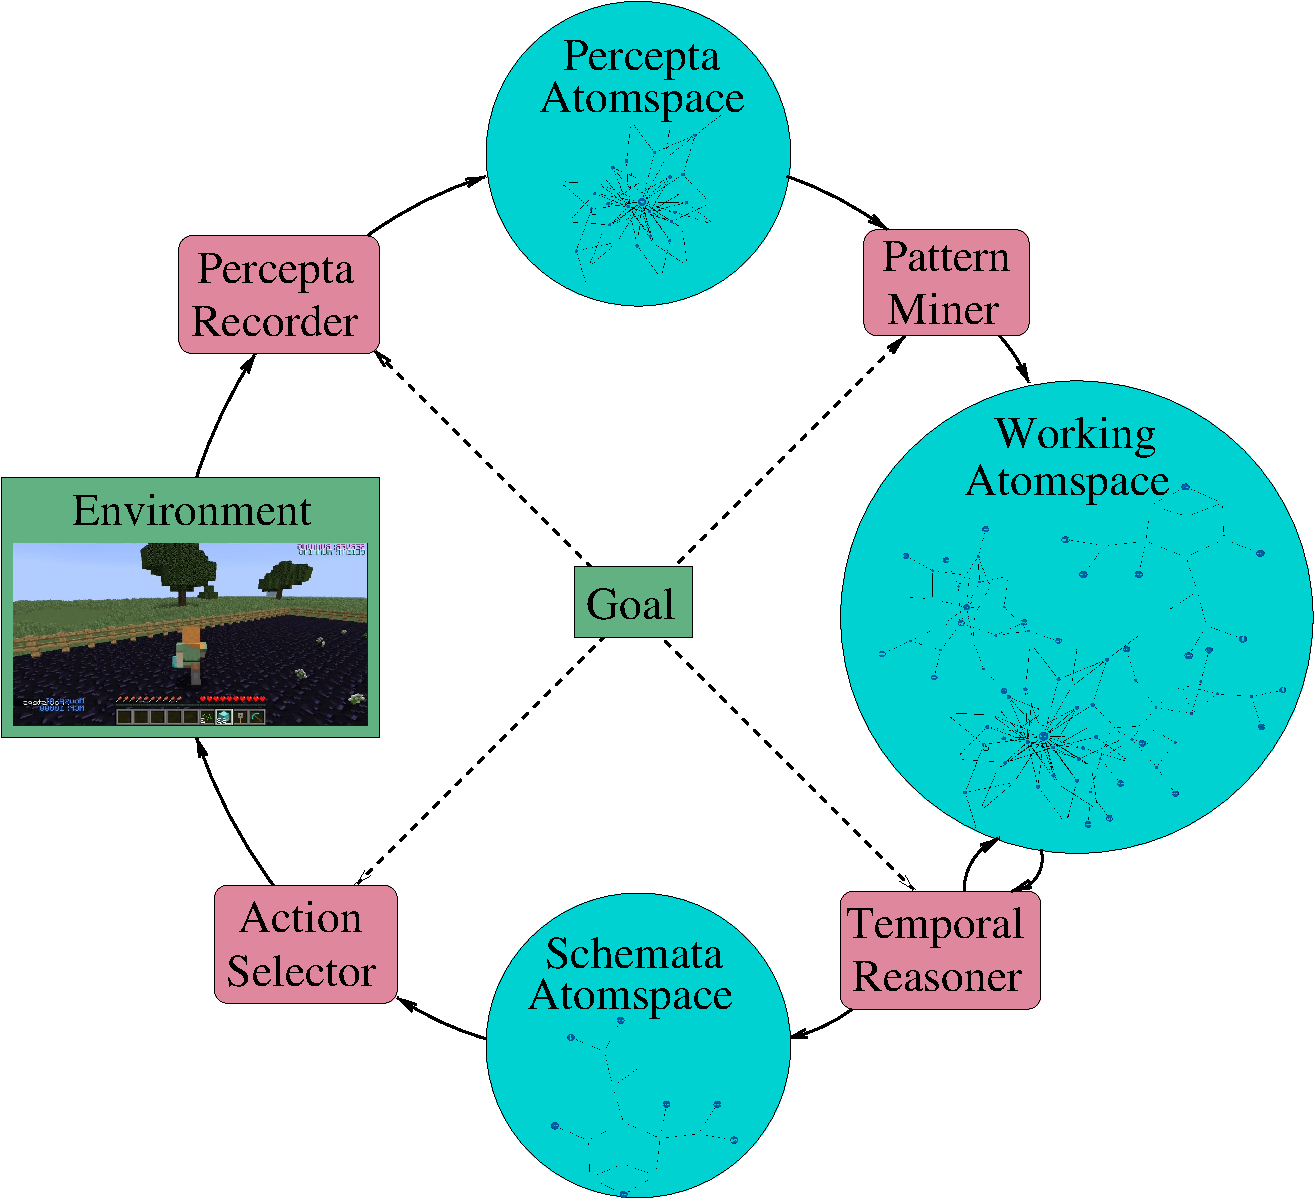
\includegraphics[width=0.54\textwidth]{pictures/rocca-chart-v0.7.pdf}
  \end{center}

\end{frame}

\section{Planning}

\subsection{Introduction}

\begin{frame}

  \begin{columns}
    \column{3.2in}
    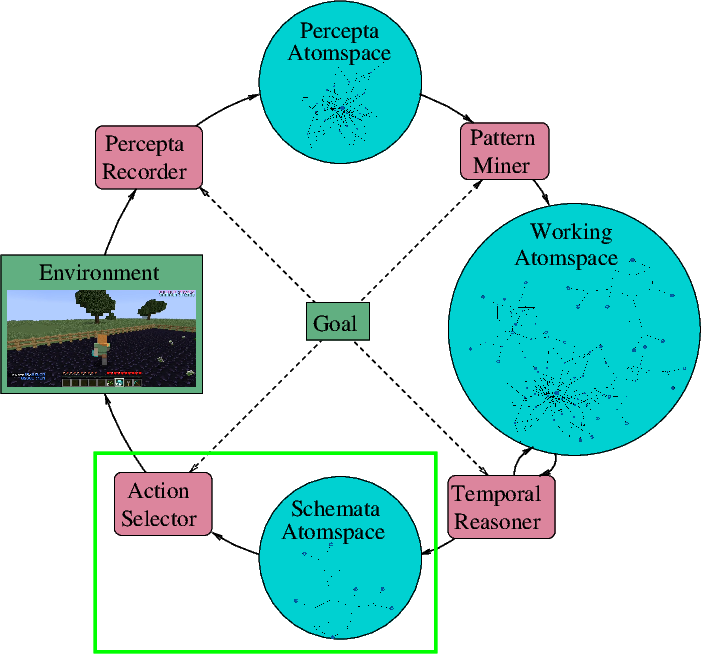
\includegraphics[scale=0.3]{pictures/rocca-chart-action-highlight-v0.7.png}
    \column{2.5in}
    \underline{Cognitive Schematic}
    \begin{itemize}
    \item $\text{Context}\ \land\ \text{Action}\ \lpreimp{T}\ \text{Goal}$
    \end{itemize}
  \end{columns}

\end{frame}

\begin{frame}

  % <BEGIN-SPEECH>
  % Everything that is turn to the past is left associative, everything
  % that is turned to the future is right associative, and that way we
  % can remove all parenthesis and read from the left to right, in
  % chronological order.
  % <END-SPEECH>

  \begin{center}
    \only<1>{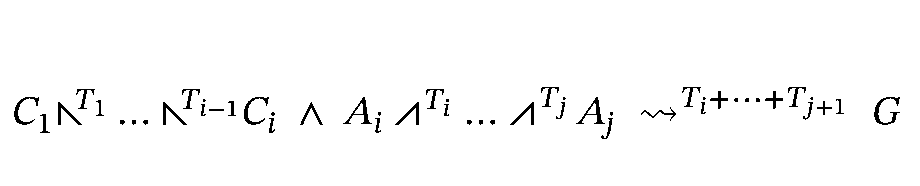
\includegraphics[scale=0.4]{pictures/schema-not-decorated.png}}
    \only<2->{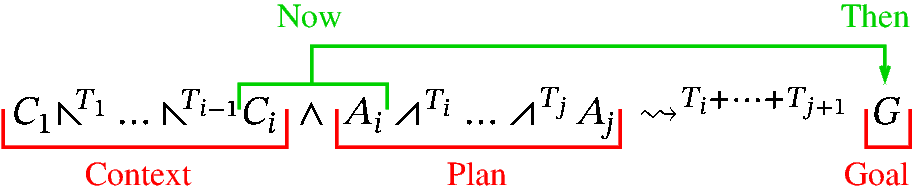
\includegraphics[scale=0.4]{pictures/schema-decorated.png}}
  \end{center}

  % <BEGIN-SPEECH>
  % Well, in a way everything is happening now, because, you remember I
  % said that this operator brings the past into the present, and that
  % one, and that one too, brings the future into the present, so
  % everything is from the viewpoint of the present.  But of course we
  % can't evaluate what is coming from the future, but everything else
  % we can.  So for instance if t is now, then we can evaluate
  % <END-SPEECH>

  \pause\pause

  {\large
    $$
    \begin{array}{ccc}
      \left[ C_1 \lbseqand{\!\! T_1} \dots \lbseqand{\!\! T_{i-1}} C_i
      \right](t) & = & \textit{True}\ |\ \textit{False}\\
      \pause & \mapsto & \mathcal{Dist}(Bool) \\
      \pause & \mapsto & \mathcal{Dist}(\mathcal{Dist}(Bool)) \\
    \end{array}
    $$
  }

  % <BEGIN-SPEECH>
  % And normally we should be able to evaluate to True or False, unless of
  % course the predicates are inherently uncertain, or we have forgotten
  % the past, etc, in which case it will be evaluated to a Bernouilli distribution,
  % possibly even a second order Bernouilli distribution.
  % <END-SPEECH>

\end{frame}

\begin{frame}
  % \frametitle{It is always now}

  % <BEGIN-SPEECH>
  % So for instance if all you've got is this schema, then in order to
  % continue the plan after taking the first action, you need to at
  % least apply temporal transposition so that the follow-up of the
  % plan is expressed from the view point of now.
  %
  % So that after selecting action A1, then A2 becomes the present
  % action, and A1 becomes the context, and then A3 becomes the
  % present action and A2 becomes the context as well.  And of course
  % you're getting closer and closer to the goal.
  % <END-SPEECH>

  % {\huge
  %   $$
  %   C \land A_1 \lseqand{T_1} A_2 \lseqand{T_2} A_3
  %   \lpreimp{T_1+T_2+T_3} G
  %   $$
  %   $$
  %   C \land A_1 \lbseqand{\!\! T_1}\ A_2 \lseqand{T_2} A_3 \lpreimp{T_2+T_3}
  %   G
  %   $$
  %   $$
  %   C \land A_1 \lbseqand{\!\! T_1} A_2 \lbseqand{\!\! T_2}\ A_3 \lpreimp{T_3} G
  %   $$
  %   }

  \begin{center}
    \only<1>{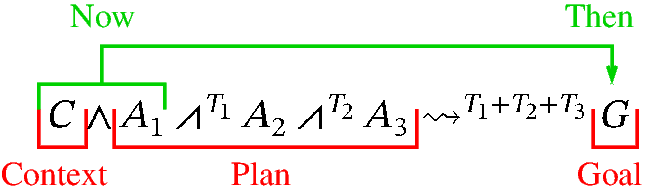
\includegraphics[scale=0.3]{pictures/C-A1A2A3-decorated.png}}
    \only<2->{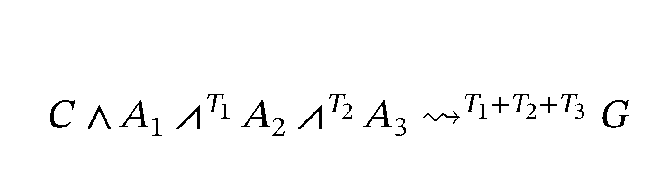
\includegraphics[scale=0.3]{pictures/C-A1A2A3-not-decorated.png}}

    % \visible<2->{\alert{$A_1\dashdownarrow T_1$}}\\

    % <BEGIN-SPEECH>
    % However we have a new schema, that is merely a temporal
    % transposition of the previous one, such that now action A2 is in
    % the present, and therefore can be selected for execution.
    % <END-SPEECH>

    \visible<2->{
      \only<-2>{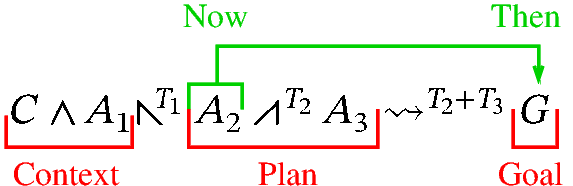
\includegraphics[scale=0.3]{pictures/CA1-A2A3-decorated.png}}
      \only<3->{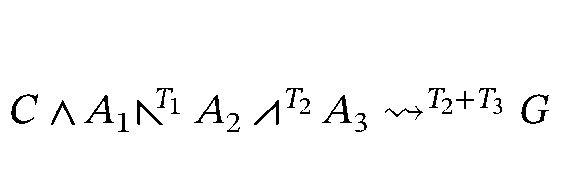
\includegraphics[scale=0.3]{pictures/CA1-A2A3-not-decorated.png}}}

    % \visible<3>{\alert{$A_2\dashdownarrow T_2$}}\\

    \visible<3>{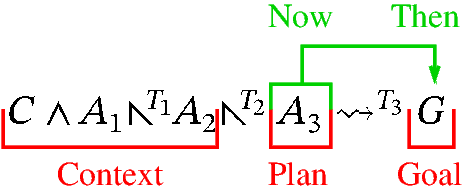
\includegraphics[scale=0.3]{pictures/CA1A2-A3-decorated.png}}
  \end{center}

\end{frame}

\subsection{Example: Collect Diamonds}

\begin{frame}
  \frametitle{Example: Collect Diamonds}
  \begin{columns}
    \column{4.4in}
    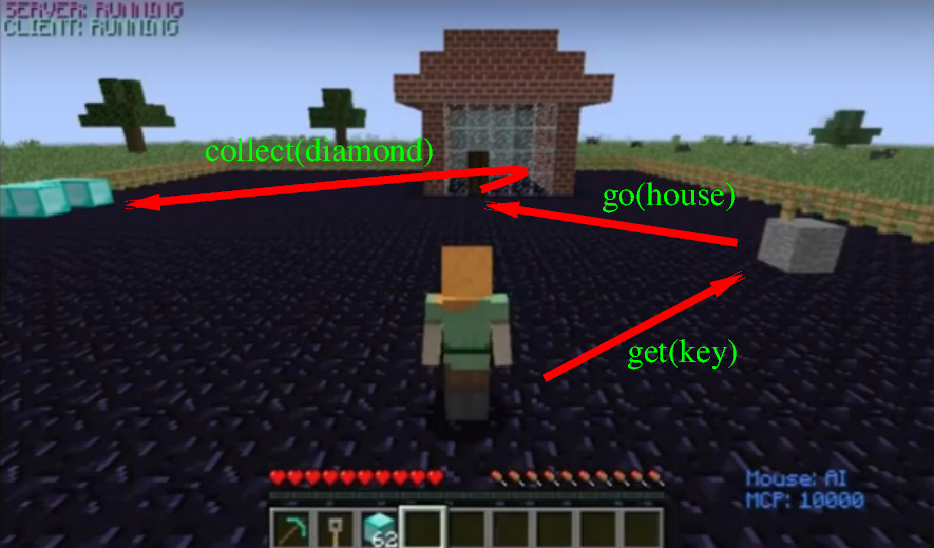
\includegraphics[scale=0.33]{pictures/minecraft-arrows.png}
    \column{1.7in}
    % \begin{itemize}
    \underline{Actions}
      \begin{itemize}
      \item get(key)
      \item go(house)
      \item collect(diamond)
      \end{itemize}
    \underline{Percepts}
      \begin{itemize}
      \item outside(house)
      \item inside(house)
      \item hold(key)
      \item next(door)
      \item reward(1)
      \item reward(0)
      \end{itemize}
    % \end{itemize}
  \end{columns}
\end{frame}

\begin{frame}
  \frametitle{Example: Collect Diamonds}

  % \begin{center}

  % <BEGIN-SPEECH>
  % We're gonna let aside the learning aspect for a moment and assume
  % we already have the correct schemata to collect diamonds, and I'm
  % gonna simulate the sequence of schemata and action selection.
  % <END-SPEECH>

  % <BEGIN-SPEECH>
  % The agent is outside of the house, and we happen to have this
  % schema that can be applied.  So it is gonna get the key
  % <END-SPEECH>

    \visible<2->{$\text{outside(house)} \land
      \text{\color<3>{mygreen}{get(key)}} \lseqand{1} \text{go(house)}
      \lseqand{1} \text{collect(diamond)} \lpreimp{3}
      \text{reward(1)}$\\[0.3cm]}

  % <BEGIN-SPEECH>
  % Now it holds the key, and we happen to have this other schema that
  % can be applied.  So it's gonna take the next possible action which
  % is to go to the house.
  % <END-SPEECH>

    \visible<4->{$\text{hold(key)} \land \text{\color<5>{mygreen}{go(house)}} \lseqand{1} \text{collect(diamond)}
      \lpreimp{2} \text{reward(1)}$\\[0.3cm]}

  % <BEGIN-SPEECH>
  % Finally the agent is inside the house, and if it collects a
  % diamond it will get a reward.
  % <END-SPEECH>

    \visible<6->{$\text{inside(house)} \land \text{\color<7>{mygreen}{collect(diamond)}} \lpreimp{1}
      \text{reward(1)}$\\[0.3cm]}

  % \end{center}

  \only<-2>{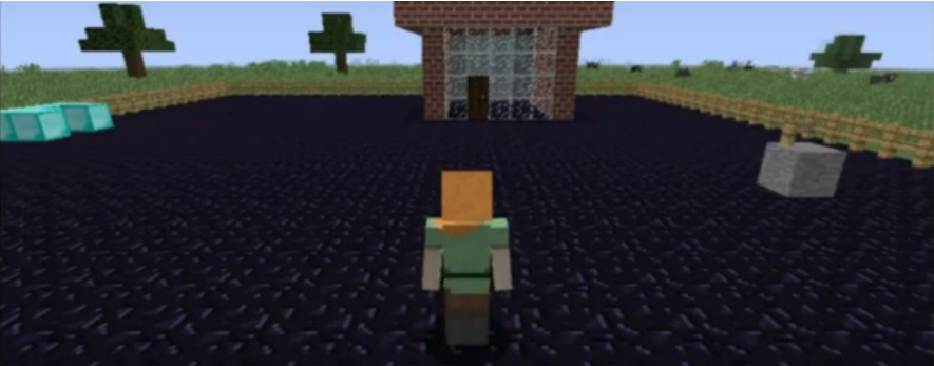
\includegraphics[scale=0.3]{pictures/minecraft-wide-no-arrow.png}}
  \only<3,4>{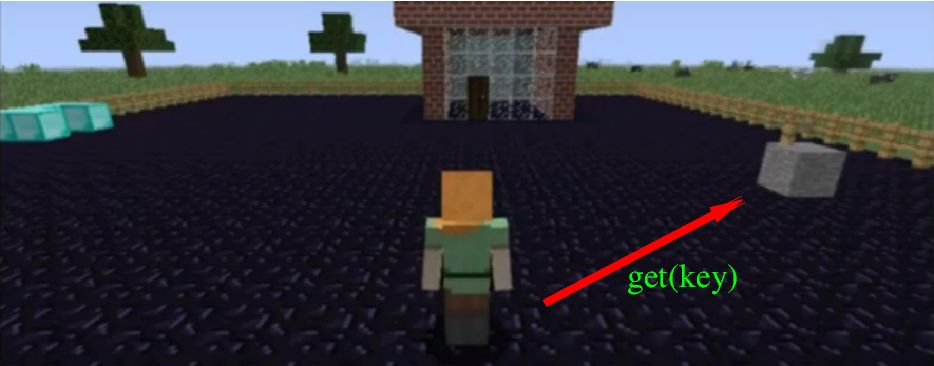
\includegraphics[scale=0.3]{pictures/minecraft-wide-1-arrow.png}}
  \only<5,6>{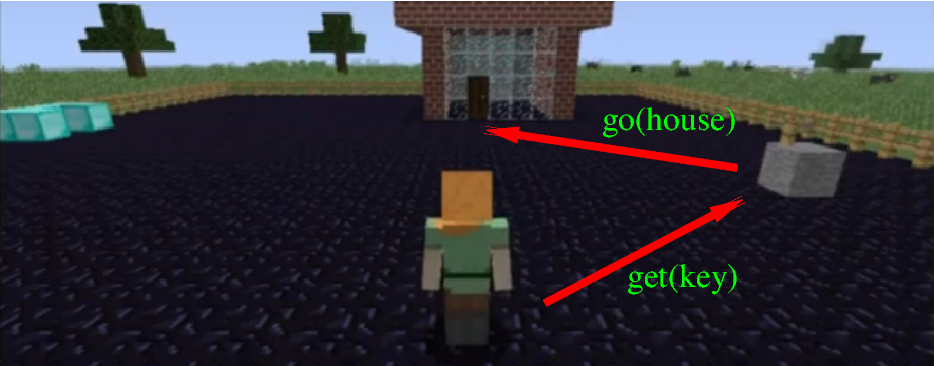
\includegraphics[scale=0.3]{pictures/minecraft-wide-2-arrows.png}}
  \only<7->{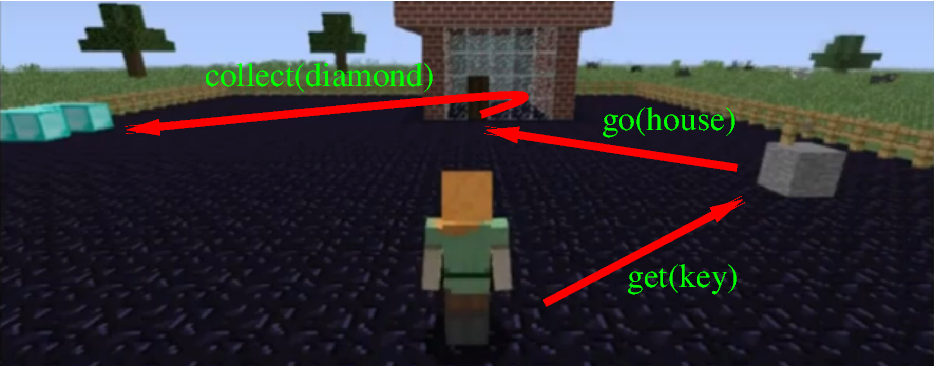
\includegraphics[scale=0.3]{pictures/minecraft-wide-3-arrows.png}}

\end{frame}

\subsection{The Paradox of Choice}

\begin{frame}
  \frametitle{The Paradox of Choice}

  % <BEGIN-SPEECH>
  % Here the best schemata were directly provided, but in reality we
  % may have hundreds, or thousands, or even millions of valid
  % schemata leading to the same goal, and we need to pick one.  Also,
  % something I haven't talk about so far, is that we have truth
  % values attached to these schemata
  % providing very different estimates about the likelihood
  % of success of their plans, sometimes even contradicting each
  % others.
  % <END-SPEECH>

  \alert{\underline{Many applicable schemata}}\\
  $$
  \begin{array}{ccc}
    C_1 \land A_1 \lpreimp{T_1} G & \measeq & \textit{TV}_1\\
    % C_2 \land A_2 \lpreimp{T_2} G & \measeq & \textit{TV}_2\\
    % C_3 \land A_3 \lpreimp{T_3} G & \measeq & \textit{TV}_3\\
    \vdots & & \\
    C_{9999} \land A_{9999} \lpreimp{T_{9999}} G & \measeq & \textit{TV}_{9999}
  \end{array}
  $$

  \pause

  % <BEGIN-SPEECH>
  % For instance we may have this and that
  % <END-SPEECH>

  \alert{\underline{Some contradicting each other}}\\
  $$
  \begin{array}{ccc}
    C_1 \land A \lpreimp{T_1} G & \measeq & <\!0.9\ 0.5\!>\\
    C_2 \land A \lpreimp{T_1} G & \measeq & <\!0.1\ 0.5\!>
  \end{array}
  $$

  \pause

  % <BEGIN-SPEECH>
  % Would you rather choose something that is very likely to succeed
  % but you not confident about?  Or something that moderately
  % likely to succeed but you're very confident about?
  % <END-SPEECH>

  \alert{\underline{With different risk/reward profiles}}\\

  $$
  \begin{array}{ccc}
    C_1 \land A_1 \lpreimp{T_1} G & \measeq & <\!0.9\ 0.1\!>\\
    C_2 \land A_2 \lpreimp{T_2} G & \measeq & <\!0.6\ 0.9\!>
  \end{array}
  $$
\end{frame}

\begin{frame}
  \frametitle{Balancing exploitation and exploration}

  % <BEGIN-SPEECH>
  % And we obtain a giant second order mixture that contains all
  % schemata, then we use Thompson Sampling over that mixture, and
  % that gives us our next action.
  % <END-SPEECH>

  \begin{center}
    Solomonoff-ish Induction  \visible<2->{\alert{$\searrow$}}  \\
    $\ \ \ \ \ \ \ \ \ \ \ \ \ \ \ \ \ \ \ \ \ \ \ \ \ \ \ \ \ \ \ \ \
    \ \ \ \ \ \ \ \ \ \ \ \ \ \ \ \ \ \ \ \ \ \ \ + \ \ \ \ \ \ \ \ \
    \ \ \ \ \ \ \ \ \ \ \ \ \ \ \ \ $
    \visible<2->{\alert{Second Order Mixture}} \\
    $\ \ \ $ Thompson Sampling $\ \ $ \visible<2->{\alert{$\swarrow$}}
  \end{center}

  \pause\pause

  % <BEGIN-SPEECH>
  % The idea of Thompson Sampling is that, if we don't exactly know,
  % we should allow ourselves to consider we are in one of the
  % probable worlds, and plan and act accordingly.
  % <END-SPEECH>

  \begin{center}
    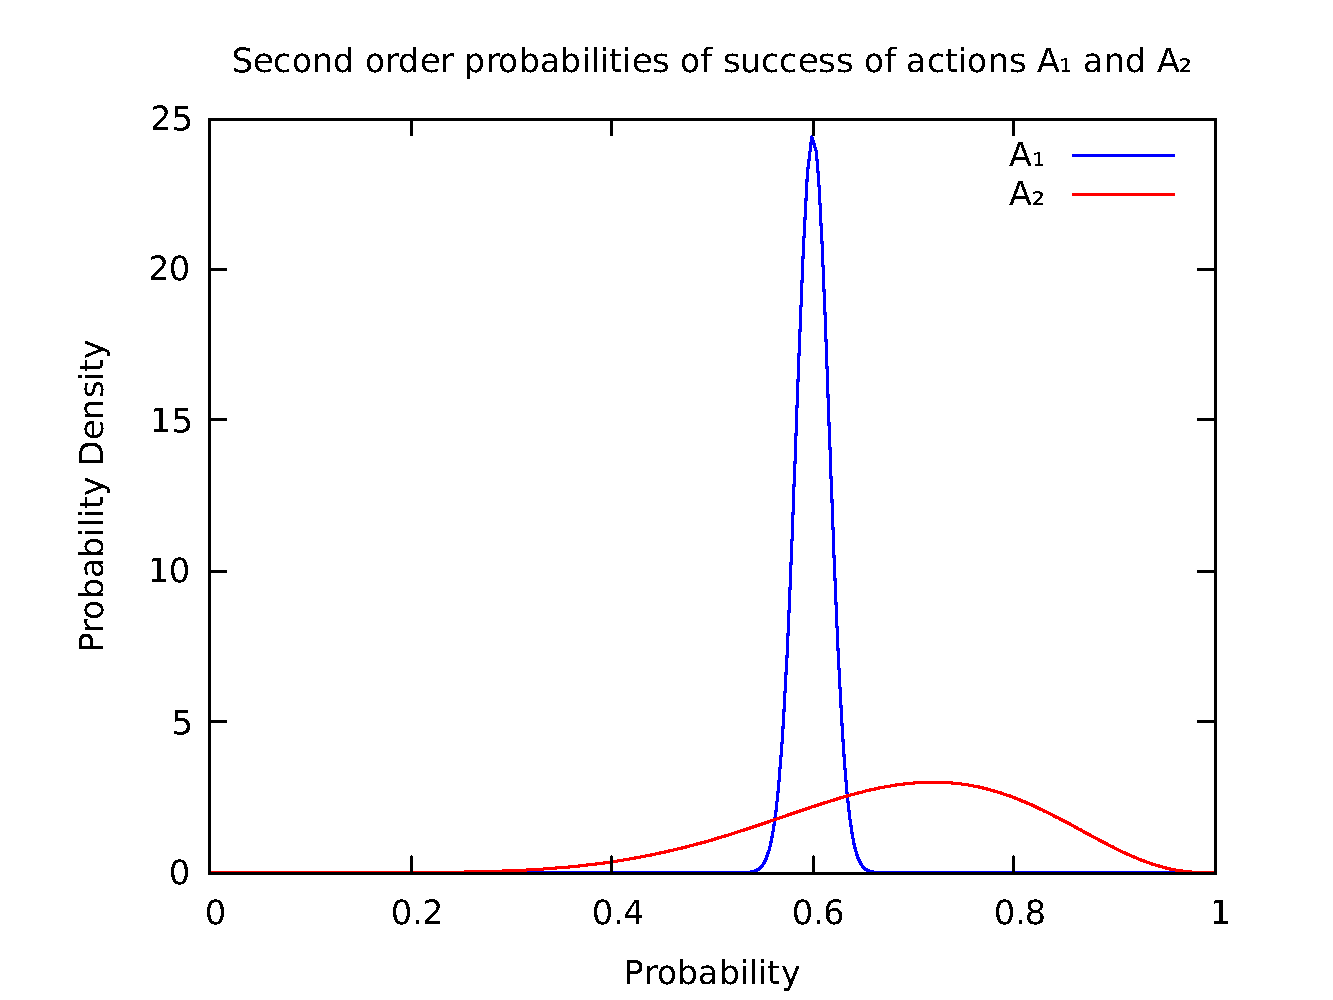
\includegraphics[scale=0.31]{pictures/actiondist.pdf}
  \end{center}

\end{frame}

\section{Learning}

\begin{frame}
  \frametitle{Learning Schemata}

  % <BEGIN-SPEECH>
  % So now I'm going to address that part, how to learn cognitive
  % schematics.  I'm gonna spend a lot of time on that cause it's been
  % covered in other publications, but basically it is currently the
  % combination of two things, Pattern Mining and Temporal/Procedural
  % Reasoning.
  % <END-SPEECH>

  \begin{columns}
    \column{3.2in}
    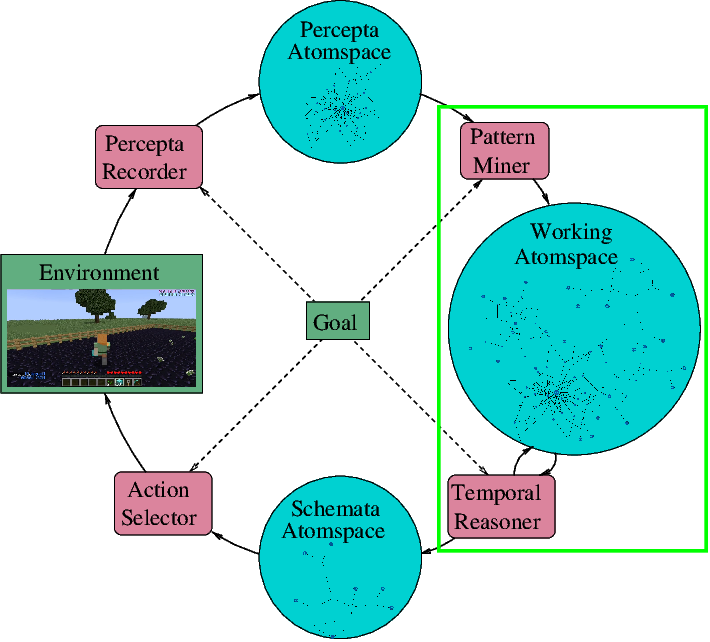
\includegraphics[scale=0.3]{pictures/rocca-chart-learning-highlight-v0.7.png}
    \column{2.5in}
    \begin{center}
      Pattern Mining\\
      +\\
      Temporal Reasoning
    \end{center}
  \end{columns}

\end{frame}

\begin{frame}
  \frametitle{Pattern Mining Schemata}

  % <BEGIN-SPEECH>
  % So, simply put, the idea of pattern mining, is that given a stream
  % of observations, we can mine simple cognitive schematics such as
  % this one, among hundreds of other patterns.  This expresses the
  % idea that if the agent holds a key and go to the house, then,
  % after one time unit, it'll end up inside the house with a decent
  % probability and a low confidence.
  % <END-SPEECH>

  \begin{columns}
    \column{3cm}
    $
    \begin{array}{|l|l|}
      \hline
      \textit{Time} & \textit{Event} \\
      \hline
      \vdots & \vdots \\
      10 & \textit{reward(0)} \\
      10 & \textit{outside(house)} \\
      10 & \textit{hold(key)} \\
      10 & \textit{go(house)} \\
      11 & \textit{inside(house)} \\
      11 & \textit{go(diamond)} \\
      11 & \textit{reward(0)} \\
      12 & \textit{reward(1)} \\
      \vdots & \vdots \\
      \hline
    \end{array}
    $
    \column{9cm}
    $
    \begin{array}{c}
      \vdots \\
      \vdots \\
      % \textit{outside(house)} \land \textit{go(key)} \lpreimp{1}
      % \textit{hold(key)} \measeq\ <\!1, 0.007\!> \\
      \vdots \\
      \textit{hold(key)} \land \textit{go(house)} \lpreimp{1}
      \textit{inside(house)} \measeq\ <\!0.833, 0.007\!> \\
      \vdots \\
      % \textit{outside(house)} \land \textit{go(key)} \lpreimp{1}
      % \textit{outside(house)} \measeq\ <\!1, 0.007\!> \\
      \vdots \\
      \vdots
    \end{array}
    $
  \end{columns}

  % <BEGIN-SPEECH>
  % But pattern mining alone is not enough.  First, because in order
  % for the mining to be tractable the expressiveness of the patterns
  % must be somewhat limited.  The miner will be able to discover
  % surprising relationships between existing entities in the
  % AtomSpace, but it won't be able to discover relationships between
  % sophisticated abstractions of these entities.  And secondly, and
  % actually it is tied to its lack of expressiveness, in order to
  % learn a complex pattern, then you're gonna need a lot of data,
  % often more than what you have.  It's a bit similar to a large
  % language model that may need to read a 1000 times more text than
  % an any human being would be able to in its entire life time, in
  % order to learn a descent approximation of natural language.  So to
  % address that problem we also use reasoning in general, and
  % temporal and procedural reasoning in particular.
  % <END-SPEECH>

\end{frame}

\begin{frame}
  \frametitle{Reasoning Schemata}

  % <BEGIN-SPEECH>
  % And then we can combine these simple schemata into more complex
  % ones via temporal reasoning.
  % <END-SPEECH>

  % {\tiny
  %   \begin{prooftree}
  %     \AxiomC{$\textit{outside(house)} \land \textit{go(key)} \lpreimp{1}
  %       \textit{outside(house)} \measeq\ <\!1, 0.007\!>$}
  %     \AxiomC{$\textit{outside(house)} \land \textit{go(key)} \lpreimp{1}
  %       \textit{hold(key)} \measeq\ <\!1, 0.007\!>$}
  %     \RightLabel{(TCC)}
  %     \BinaryInfC{$\textit{outside(house)} \land \textit{go(key)} \lpreimp{1}
  %       \textit{outside(house)} \land \textit{hold(key)} \measeq\
  %       <\!1, 0.007\!>$}

  %     \AxiomC{$\textit{outside(house)} \land \textit{hold(key)}
  %       \land \textit{go(house)} \lpreimp{1} \textit{inside(house)}
  %       \measeq\ <\!0.833, 0.007\!>$}
  %     \RightLabel{PD}
  %     \BinaryInfC{$\textit{outside(house)} \land \textit{go(key)} \lseqand{1} \textit{go(house)} \lpreimp{2} \textit{inside(house)} \measeq\ <\!0.833, 0.007\!>$}
  %   \end{prooftree}
  % }

  {\tiny
    \begin{prooftree}
      \AxiomC{$\!\!\!\!\!\textit{outside(house)} \land \textit{go(key)} \lpreimp{1}
        \textit{outside(house)}\!\!\!\!\!$}
      \AxiomC{$\!\!\!\!\!\textit{outside(house)} \land \textit{go(key)} \lpreimp{1}
        \textit{hold(key)}\!\!\!\!\!$}
      \RightLabel{(CC)}
      \BinaryInfC{$\!\!\!\!\!\textit{outside(house)} \land \textit{go(key)} \lpreimp{1}
        \textit{outside(house)} \land \textit{hold(key)}\!\!\!\!\!$}

      \AxiomC{$\!\!\!\!\!\textit{outside(house)} \land \textit{hold(key)}
        \land \textit{go(house)} \lpreimp{1} \textit{inside(house)}\!\!\!\!\!$}
      \RightLabel{(PD)}
      \BinaryInfC{$\!\!\!\!\!\textit{outside(house)} \land \textit{go(key)} \lseqand{1} \textit{go(house)} \lpreimp{2} \textit{inside(house)}\!\!\!\!\!$}
    \end{prooftree}
  }

  \pause

  {\small $$\vdots$$}

  {\tiny
    $$\textit{outside(house)} \land \textit{go(key)} \lseqand{1}
    \textit{go(house)} \lseqand{1} \textit{go(diamond)} \lpreimp{3}
    \textit{reward(1)} \measeq\ <\!0.833, 0.005\!>$$
  }

  % <BEGIN-SPEECH>
  % If we wanted to get this schema with pattern mining alone, we
  % could.  However, you can see it involve a sequence of 3 actions,
  % and so in order to discover this sequence via pattern mining we
  % would the agent to take it, so it can be observed, ideally more
  % than once, in order to have a decent confidence.  But that's the
  % optimal sequence of actions, in that context that is, so we'd have
  % to stumble by change on the optimal sequence of actions in order
  % to form a plan for of sequence, which, in general you can guess,
  % is extremely unlikely.  So that is exactly what reasoning brings
  % us, we don't need to wait to stumble on a plan to make an
  % educated guess about its likelihood of success.
  % <END-SPEECH>

\end{frame}

\section{Perception}

\begin{frame}

  % <BEGIN-SPEECH>
  % And for the observation phase, all percepts coming from the
  % environment are mechanically timestamped and stored in the
  % Percepta AtomSpace.  I know that in general perception should not
  % be treated independently from cognition, but that's how it works
  % for now.  The format does not matter, what matters is that in the
  % end, it can be interpreted as a temporal predicate evaluations
  % because that is what we need for pattern mining and reasoning.
  % And the absence of observation counts as its negation.
  % <END-SPEECH>

  \begin{columns}
    \column{3.2in}
    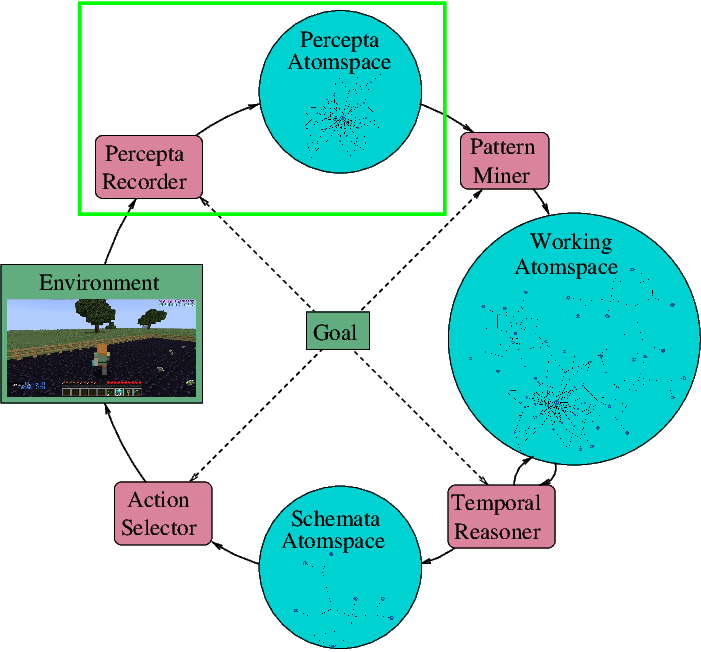
\includegraphics[scale=0.3]{pictures/rocca-chart-perception-highlight-v0.7.png}
    \column{2.5in}
    \underline{Timestamped Recorded Events}:

    {\tiny
    $
    \begin{array}{|l|l|l|}
      \hline
      \textit{Time} & \textit{Event} & \textit{Evaluation} \\
      \hline
      \vdots & \vdots & \vdots \\
      10 & \textit{reward(0)} & \textit{reward(0)(10)}=\textit{True} \\
      10 & \textit{outside(house)} & \textit{outside(house)(10)}=\textit{True} \\
      10 & \textit{hold(key)} & \textit{hold(key)(10)}=\textit{True} \\
      10 & \textit{go(house)} & \textit{go(house)(10)}=\textit{True} \\
      11 & \textit{inside(house)} & \textit{inside(house)(11)}=\textit{True} \\
      11 & \textit{go(diamond)} & \textit{go(diamond)(11)}=\textit{True} \\
      11 & \textit{reward(0)} & \textit{reward(0)(11)}=\textit{True}\\
      12 & \textit{reward(1)} & \textit{reward(1)(12)}=\textit{True}\\
      \vdots & \vdots & \vdots \\
      \hline
    \end{array}
    $}

  \end{columns}
\end{frame}

\begin{frame}
  \frametitle{Future Work}
  \begin{itemize}
  \item Attention Allocation
  \item Concept creation and schematization
  \item Plan in the inner world
  \end{itemize}
\end{frame}

\end{document}
